\documentclass[hidelinks,a4paper,12pt, nofootinbib]{article}
\usepackage[width=15.5cm, left=3cm, top=2.5cm, right=2cm, left=2cm, height= 24.5cm]{geometry}
\usepackage[spanish, es-tabla]{babel} %es-tabla es para que ponga Tabla en vez de Cuadro en el caption
\usepackage[utf8]{inputenc}
\usepackage[T1]{fontenc}
\usepackage{xspace}
\usepackage{xargs}
\usepackage{fancyhdr}
\usepackage{lastpage}
\usepackage{caratula}
\usepackage[bottom]{footmisc}
\usepackage{amsmath}
\usepackage{amssymb}
\usepackage{algorithm}
\usepackage[noend]{algpseudocode}
\usepackage{array}
\usepackage{xcolor,colortbl}
\usepackage{amsthm}
\usepackage{listings}
\usepackage{soul}

\usepackage{pgf}
\usepackage{tikz}
\usetikzlibrary{arrows,automata}

\usepackage{graphicx}
\usepackage{sidecap}
\usepackage{amsmath}
\usepackage{wrapfig}
\usepackage{caption}

\usepackage{hyperref}
\hypersetup{
  colorlinks   = true, %Colours links instead of ugly boxes
  urlcolor     = blue, %Colour for external hyperlinks
  linkcolor    = blue, %Colour of internal links
  citecolor   = red %Colour of citations
}

\usepackage{comment}

\usepackage[
  backend=bibtex,
  style=alphabetic
]{biblatex}
\addbibresource{bibliografia.bib}


\captionsetup[table]{labelsep=space}


\setlength{\parindent}{4em}
\setlength{\parskip}{0.5em}

%Defino colores para las tablas
\definecolor{LightCyan}{rgb}{0.77,0.9,0.9}
\definecolor{Gray}{gray}{0.8}


%%fancyhdr
\pagestyle{fancy}
\thispagestyle{fancy}
\addtolength{\headheight}{1pt}
\lhead{Aalgoritmos y Estructuras de Datos III: TP2}
\rhead{$1º$ cuatrimestre de 2016}
\cfoot{\thepage\ / \pageref{LastPage}}
\renewcommand{\footrulewidth}{0.4pt}
\renewcommand{\labelitemi}{$\bullet$}

%%caratula
\materia{Algoritmos y Estructuras de Datos III}
\titulo{Trabajo Práctico Número 2}
%\subtitulo{}
%\grupo{Grupo 12}
\integrante{Ciruelos Rodríguez, Gonzalo}{063/14}{gonzalo.ciruelos@gmail.com}
\integrante{Costa, Manuel José Joaquín}{035/14}{manucos94@gmail.com}
\integrante{Gatti, Mathias Nicolás}{477/14}{mathigatti@gmail.com}
\integrante{Maddonni, Axel Ezequiel}{200/14}{axel.maddonni@gmail.com}

\fecha{8 de Abril de 2016}

\usepackage{etoolbox}
\AtBeginEnvironment{tikzpicture}{\shorthandoff{>}\shorthandoff{<}}{}{}

\begin{document}
\maketitle

\tableofcontents
\newpage

\section{Una Nueva Esperanza}
\subsection{Explicación formal del problema}

\subsection{Explicación de la solución}

\subsubsection{Explicación del código}

\subsubsection{Pseudocódigo}

\subsubsection{Correctitud}

\subsubsection{Optimalidad}

\subsection{Complejidad del algoritmo}

\subsubsection{Complejidad en peor caso}

\subsubsection{Complejidad en mejor caso}

\subsection{Performance del algoritmo}

\subsubsection{M\'etodo de experimentación}
\newpage

\section{El Imperio Contraataca}
\subsection{Explicación formal del problema}

\subsection{Explicación de la solución}

\subsubsection{Explicación del código}

\subsubsection{Pseudocódigo}

\subsubsection{Correctitud}

\subsubsection{Optimalidad}

\subsection{Complejidad del algoritmo}

\subsubsection{Complejidad en peor caso}

\subsubsection{Complejidad en mejor caso}

\subsection{Performance del algoritmo}


\begin{figure}[H]
 \centering
	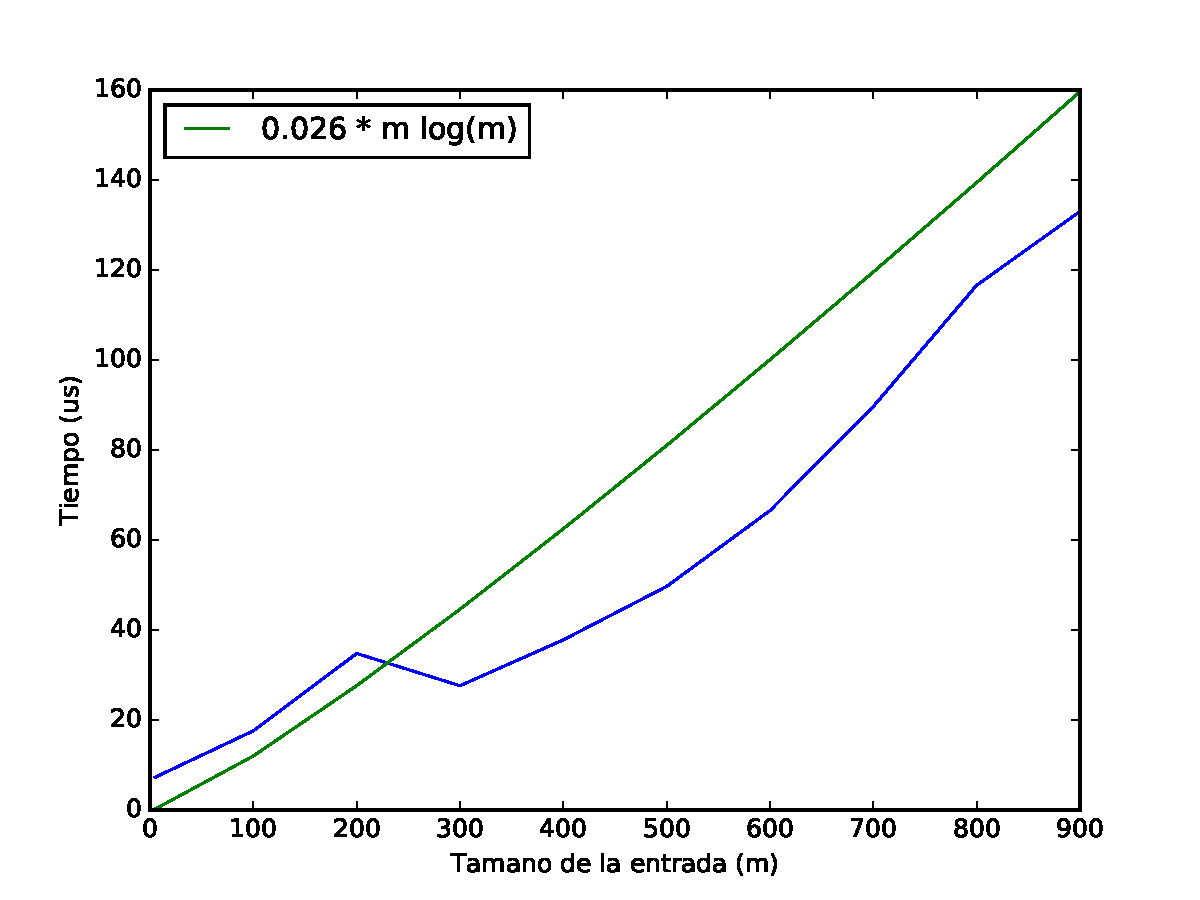
\includegraphics[width=0.8\textwidth]{img/exp/problema2-promedio.pdf}
	\caption{\footnotesize Tiempo que toma el algoritmo en $\mu$s para una entrada de tamaño $m$. $n$ al azar.}
	\label{fig:problema2-promedio}
\end{figure}

\begin{figure}[H]
 \centering
	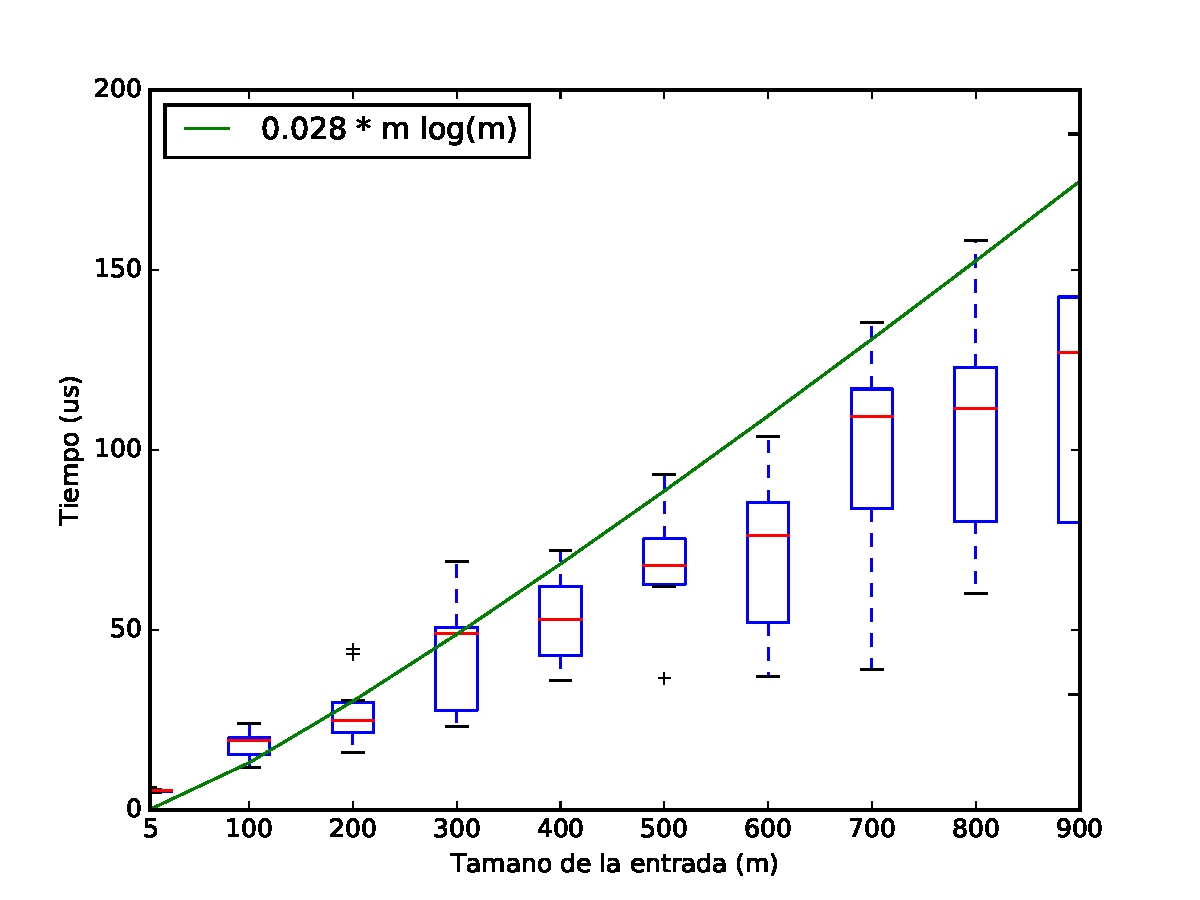
\includegraphics[width=0.8\textwidth]{img/exp/problema2-promedio2.pdf}
  \caption{\footnotesize Tiempo que toma el algoritmo en $\mu$s para una entrada de tamaño $m$. $n$ al azar. Se indican los valores del primer al tercer cuartil con un rectángulo azul y la mediana con una linea roja. El máximo y minimo se indican con lineas negras arriba y abajo del rectángulo.}
	\label{fig:problema2-promedio2}
\end{figure}

\begin{figure}[H]
 \centering
	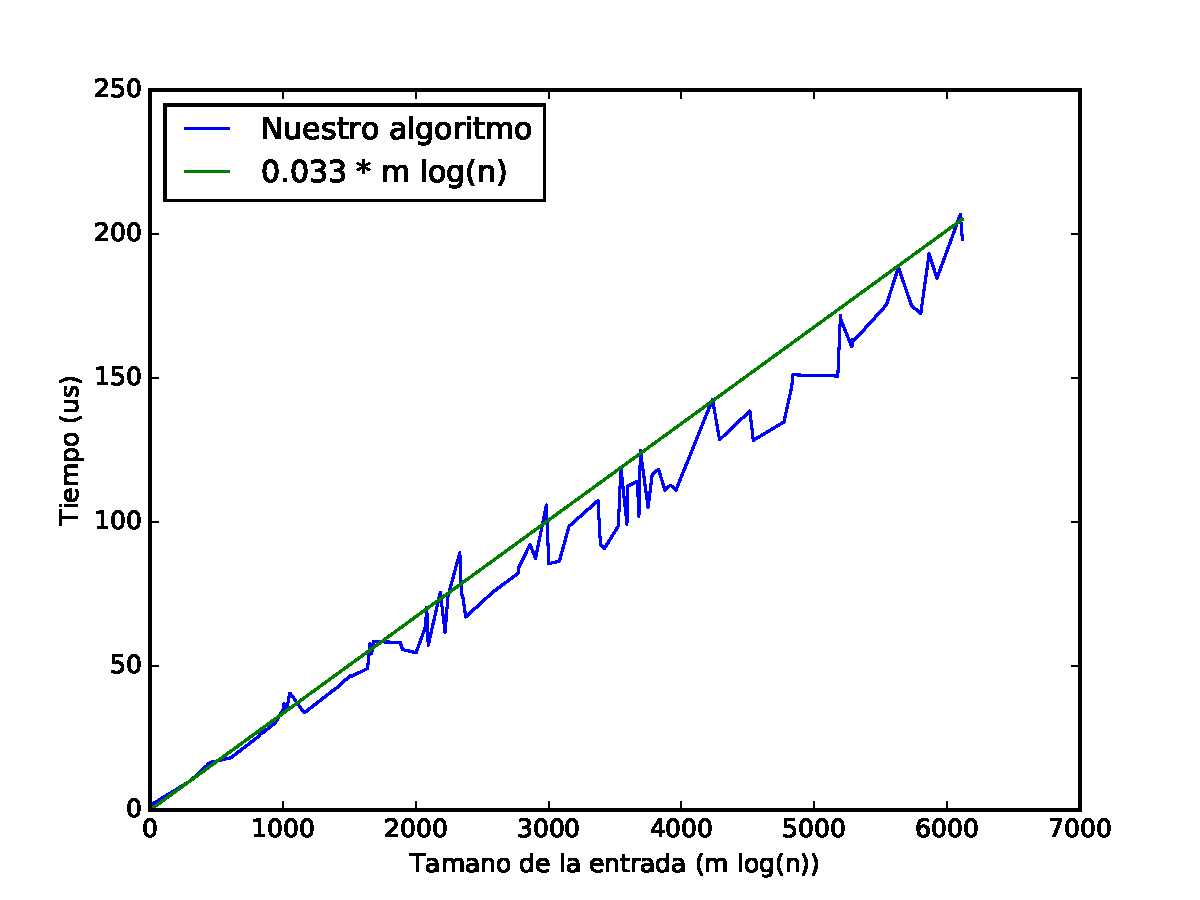
\includegraphics[width=0.8\textwidth]{img/exp/problema2-posta.pdf}
	\caption{\footnotesize Tiempo que toma el algoritmo en $\mu$s para una entrada de tamaño $m \log n$.}
	\label{fig:problema2-posta}
\end{figure}


\subsubsection{M\'etodo de experimentación}


\newpage

\section{ El Retorno del \texorpdfstring{\st{que te}} \\ Jedi}
\subsection{Explicación formal del problema}

\subsection{Explicación de la solución}

\subsubsection{Explicación del código}

\subsubsection{Pseudocódigo}

\subsubsection{Correctitud}

\subsubsection{Optimalidad}

\subsection{Complejidad del algoritmo}

\subsubsection{Complejidad en peor caso}

\subsubsection{Complejidad en mejor caso}

\subsection{Performance del algoritmo}

\subsubsection{M\'etodo de experimentación}
\newpage
\section{Apéndice}

\subsection{Generación de grafos conexos aleatorios}
\label{subsec:grafos-aleatorios}

\begin{algorithm}[H]
  \begin{algorithmic}[1]
  \caption{Pseudocódigo del procedimiento para generar grafos conexos al azar}
  \label{algo:ap-1}
    \Procedure{grafo\_random}{\texttt{int} $n$, \texttt{int} $m$}$\rightarrow$ \texttt{Grafo}

    	\State $k_n \gets \{(0,1), (0,2), ..., (0,n), (1,2), (1,3), ..., (n-2, n-1)\}$
      \State $vertices \gets \{random.range(0, n)\}$ \Comment Empiezo con un vértice al azar
      \State $agm \gets \{\}$
      \While{$vertices$.size() $< n$}
         \State $aristas \gets$ ``aristas $(u,v)$ de $k_n$ tal que $u \in vertices$ y $v \not\in vertices$ o viceversa''
         \State $arista\_nueva \gets$ random.choice($aristas$)
         \State $agm.add(arista\_nueva)$
         \State $k_n.remove(arista\_nueva)$
         \State $vertices.add($``extremo de $arista\_nueva$ que no estaba en vertices''$)$
      \EndWhile
      \State \Comment Cuando termina este ciclo tenemos un árbol de $n$ vertices y $n-1$ aristas
      \State $grafo \gets agm$
      \While{$grafo$.size() $< m$}
         \State $arista \gets random.choice(k_n)$
         \State $grafo.add(arista)$
         \State $k_n.remove(arista)$
      \EndWhile
      \For{$arista \in grafo$}
         \State{$peso(arista) \gets random.random()$}
      \EndFor
      \Return $grafo$
		\EndProcedure
	\end{algorithmic}
\end{algorithm}


El algoritmo, se basa en generar un grafo conexo minimal (es decir, un árbol) de $n$ vértices.
Para lograr esto, técnicamente lo que hacemos es empezar con $K_n$, es decir, el grafo completo de $n$ vértices, con todos sus aristas de igual peso, y le encontramos un árbol generador mínimo utilizando Prim. Todo esto es obviamente trivial en este caso, dado que todas las aristas tienen igual peso, así que básicamente lo que hacemos es elegir una arista al azar en cada paso.

Luego, una vez que tenemos el árbol terminado, lo completamos con aristas al azar, hasta llegar al objetivo de $m$ aristas. 

Finalmente, se eligen pesos al azar para cada arista.


\newpage
\subsection{Partes relevantes del código}
\lstset{language=C++, breaklines=true, basicstyle=\footnotesize}
\lstset{numbers=left, numberstyle=\tiny, stepnumber=1, numbersep=5pt, tabsize=2}

\subsubsection{problema1.cpp}
\begin{lstlisting}[frame=single]

#include <iostream>
#include <queue>
#include <vector>

using namespace std;
typedef int vertice;
typedef vector<vertice> VerticesAdyacentes;
typedef vector<VerticesAdyacentes> ListaAdyacencia;

vector<vertice> bfs(ListaAdyacencia vs, vertice root, vertice target, int n) {
  queue<vertice> c;
  vector<int> distancia(n, -1); 
  vector<int> acm(n, -1);
  vertice actual;
  distancia[root] = 0;
  acm[root] = root;
  c.push(root);
  while (!c.empty()) {
    actual = c.front();   
    c.pop();
    VerticesAdyacentes vecinos = vs[actual];
    for (const vertice& v : vecinos) {
      if (distancia[v] == -1) {
        distancia[v] = distancia[actual]+1;
        acm[v] = actual;
        if(v == target) break;
        c.push(v);
      }
    }
  }
  //Tengo que reconstruir el camino de atras 
  //para adelante
  int long_sol = distancia[target]-1;
  vector<vertice> solucion(long_sol, 0);
  //Arranco en el padre del nodo n-1
  vertice v = acm[target];

  for (int i = long_sol - 1; i >= 0; i--) {
    solucion[i] = v;
    v = acm[v];
  }

  return solucion;
}


int main() {
  int n, m;
  cin >> n >> m;
  vector<vector<int>> input;
  for (int i = 0; i < m; i++) {
    int ai, bi, ei;
    cin >> ai >> bi >> ei;
    input.push_back(vector<int>({ai, bi, ei}));
  }

  ListaAdyacencia adj_list(3*n, VerticesAdyacentes());
  for (const vector<int>& arista : input) {
    int ai = arista[0], bi = arista[1];
    bool ei = arista[2];
    if (ei) {
      adj_list[ai].push_back(bi + n);
      adj_list[ai + n].push_back(bi + 2*n);
      adj_list[bi].push_back(ai + n);
      adj_list[bi + n].push_back(ai + 2*n);
    } else {
      adj_list[ai].push_back(bi);
      adj_list[bi].push_back(ai);
      adj_list[ai + n].push_back(bi + n);
      adj_list[bi + n].push_back(ai + n);
    }

    adj_list[ai + 2*n].push_back(bi + 2*n);
    adj_list[bi + 2*n].push_back(ai + 2*n);
  }

  vector<vertice> solucion = bfs(adj_list, 0, 3*n-1, 3*n);
  
  cout << solucion.size() + 1 << endl;
  for (const int s : solucion) {
    cout << s % n << " ";
  }
  cout << endl;
}
\end{lstlisting}




\subsubsection{problema2.h}
\begin{lstlisting}[frame=single]
#include <iostream>
#include <utility>
#include <vector>

struct Vertex {
  int key;
  int value;
};

// Para facilitar la lectura. El primer elemento es el otro vertice, y el
// segundo elemento es el costo de esa ruta.
typedef std::vector<std::pair<int, int>> VerticesAdyacentes;

// MinHeap de Vertices. Es la implementacion standard, solo que con algunos 
// detalles cambiados. Hubo que agregar el arreglo "pos" que nos permite hacer
// DecValue de manera rapida (logn). No implementamos funciones de insercion
// porque no hacen falta.
class MinHeap {
 public:
  MinHeap(const std::vector<Vertex>& v);

  inline Vertex Top() const;

  Vertex Pop();

  void DecValue(int i, int new_value);

  inline size_t Size() const;

  inline int At(int i) const {
    return pos[i] >= 0;
  }

  inline int Value(int i) const {
    return a[pos[i]].value;
  }

 private:
  inline int parent(int i) { return (i - 1) / 2; }
  inline int left(int i) { return 2 * i + 1; }
  inline int right(int i) { return 2 * i + 2; }

  template <typename X>
  inline void swap(std::vector<X>& a, int i, int j) {
    X temp = a[i]; a[i] = a[j]; a[j] = temp;
  }

  template <typename X>
  inline bool inbound(std::vector<X>& a, int i) {
    return i < (int) a.size();
  }
  
  void MinHeapify(int i);

  // Array interno.
  std::vector<Vertex> a;
  // Posiciones de los elementos. Invariante: a[pos[i]].key = i.
  std::vector<int> pos;
};
\end{lstlisting}




\subsubsection{problema2.cpp}
\begin{lstlisting}[frame=single]
#include "problema2.h"

#include <cstddef>
#include <limits>

// Funcion para debugear.
void printVertexVector(std::vector<Vertex>& vs) {
  std::cerr << "{";
  for(const Vertex& v : vs) {
    std::cerr << "(" << v.key<< ", " << v.value << "), ";
  }
  std::cerr << "}" << std::endl;
}

MinHeap::MinHeap(const std::vector<Vertex>& v)
  : a(v), pos(v.size(), 0) {
  for (int i = a.size() / 2; i >= 0; i--) {
    MinHeapify(i);
  }
  for (int i = 0; inbound(a, i); i++) {
    pos[a[i].key] = i;
  }
}

Vertex MinHeap::Top() const {
  return a[0];
}

Vertex MinHeap::Pop() {
  Vertex minimum = a[0];
  // El primero deja de existir.
  pos[a[0].key] = -1;
  // El ultimo pasa a estar arriba de todo.
  pos[a[a.size() - 1].key] = 0;

  // El ultimo pasa estar arriba de todo.
  a[0] = a[a.size() - 1];
  // Achico el vector.
  a.resize(a.size() - 1);
  
  // Bajo la raiz hasta dejarlo todo bien.
  MinHeapify(0);
  return minimum;
}

void MinHeap::DecValue(int v, int new_value) {
    // Consigo el indice de v.
    int i = pos[v];
    // Le pongo el nuevo valor.
    a[i].value = new_value;
 
    // Voy para arriba "heapificando" el array.
    while (i > 0 && a[i].value < a[parent(i)].value) {
        // Lo cambio con su padre.
        pos[a[i].key] = parent(i);
        pos[a[parent(i)].key] = i;
        swap(a, i, parent(i));
        i = parent(i);
    }
}

inline size_t MinHeap::Size() const {
  return a.size();
}

void MinHeap::MinHeapify(int i) {
    int smallest = i;
    int l = left(i);
    int r = right(i);

    if (inbound(a, l) && a[l].value < a[smallest].value)
      smallest = l;
    if (inbound(a, r) && a[r].value < a[smallest].value)
      smallest = r;
 
    if (smallest != i) { 
        // Los vertices que tengo que cambiar.
        Vertex smallest_vertex = a[smallest];
        Vertex index_vertex = a[i];
        // Cambio las posiciones.
        pos[smallest_vertex.key] = i;
        pos[index_vertex.key] = smallest;
        // Cambio los vertices.
        swap(a, smallest, i);
        // Aplico MinHeapify para abajo.
        MinHeapify(smallest);
    }
}

std::vector<std::pair<int, int>> prim(
    MinHeap& heap, std::vector<VerticesAdyacentes> adj_list) {
  std::vector<std::pair<int, int>> parent(heap.Size(), std::make_pair(0, 0));

  while (heap.Size() > 0) {
    Vertex min_vertex = heap.Pop();
    int u = min_vertex.key;

    for (const auto& vertex_and_weight :  adj_list[u]) {
      int v = vertex_and_weight.first;
      int weight = vertex_and_weight.second;
      if (heap.At(v) && weight < heap.Value(v)) {
        parent[v].first = u;
        parent[v].second = weight;
        heap.DecValue(v, weight);
      }
    }
  }
  return std::move(parent);
}


int main() {
  int n, m;
  std::cin >> n >> m;
  std::vector<VerticesAdyacentes> adj_list(n, VerticesAdyacentes());

  for (int i = 0; i < m; i++) {
    int ai, bi, li;
    std::cin >> ai >> bi >> li;
    adj_list[ai].push_back(std::make_pair(bi, li));
    adj_list[bi].push_back(std::make_pair(ai, li));
  }

  std::vector<Vertex> v_inicial;
  v_inicial.push_back({.key = 0, .value = 0});
  for (int i = 1; i < n; i++) {
    v_inicial.push_back({.key = i, .value = std::numeric_limits<int>::max()});
  }
  MinHeap h(v_inicial);  
  std::vector<std::pair<int, int>> resultado = prim(h, adj_list);

  int litros = 0;
  for (const auto& x : resultado) {
    litros += x.second;
  }

  std::cout << litros << std::endl;
  for (size_t i = 1; i < resultado.size(); i++) {
    std::cout << resultado[i].first << std::endl;
  }
}
\end{lstlisting}


\subsubsection{problema3.cpp}
\begin{lstlisting}[frame=single]
#include <algorithm> // min
#include <iostream>
#include <list>
#include <tuple>
#include <vector>

using namespace std;

// La tupla corresponde a: (altura, costoMinimo, Mov: X o Z)
typedef tuple<int, int, char> Casilla;

// Definiciones
int solve(vector<vector<Casilla>>& t, int n, int m, int h);
int costo (const vector<vector<Casilla>>& t, int h, int i, int j, int k, int l);

int costocolumna(const vector<vector<Casilla>>& t, int h, int i, int j);
int costofila(const vector<vector<Casilla>>& t, int h, int i, int j);

int main() {
  int n, m, h;
  cin >> n >> m >> h;

  vector<vector<Casilla>> Tablero(n, vector<Casilla>(m, Casilla()));

  for (int i = 0; i < n; i++) {
    for (int j = 0; j < m; j++) {
      cin >> get<0>(Tablero[i][j]);
    }
  }

  int resultado = solve(Tablero, n, m, h);
  // Armo el camino minimo.
  list<char> camino;
  int i = n - 1;
  int j = m - 1;
  while (!(i == 0 && j == 0)) {
    const char mov = get<2>(Tablero[i][j]);
    camino.push_front(mov);
    mov == 'Y' ? j-- : i--;
  }

  cout << resultado << endl;
  for (const char mov : camino)
    cout << mov << endl;

  return 0;
}


int costo(const vector<vector<Casilla>>& t, int h, int i, int j, int k, int l){
  int delta = abs(get<0>(t[i][j]) - get<0>(t[k][l]));
  return delta <= h ? 0 : delta - h;
}

int costofila(const vector<vector<Casilla>>& t, int h, int i, int j) {
  return get<1>(t[i-1][j]) + costo(t, h, i-1, j, i, j);
}

int costocolumna(const vector<vector<Casilla>>& t, int h, int i, int j) {
  return get<1>(t[i][j-1]) + costo(t, h, i, j-1, i, j);
}


int solve(vector<vector<Casilla>>& t, int n, int m, int h) {
  get<1>(t[0][0]) = 0;

  for (int j=1; j < m; j++){
    get<1>(t[0][j]) = costocolumna(t, h, 0, j);
    get<2>(t[0][j]) = 'Y';
  }

  for (int i=1; i < n; i++){
    get<1>(t[i][0]) = costofila(t, h, i, 0);
    get<2>(t[i][0]) = 'X';
  }

  for (int i = 1 ; i < n; i++){
    for (int j = 1; j < m; j++){
      get<1>(t[i][j]) = min(costofila(t, h, i, j), costocolumna(t, h, i, j));
      if (get<1>(t[i][j]) == costofila(t, h, i, j))
        get<2>(t[i][j]) = 'X';
      else
        get<2>(t[i][j]) = 'Y';
    }
  }

  return get<1>(t[n-1][m-1]);
}
\end{lstlisting}


\end{document}
